\documentclass[12pt]{article}
\usepackage[margin=1in]{geometry}
\usepackage{times}
\usepackage[T1]{fontenc}
\usepackage[utf8]{inputenc}
\usepackage{amsmath,amssymb}
\usepackage{booktabs}
\usepackage{graphicx}
\usepackage{subcaption}
\usepackage{parskip}
\usepackage[numbers,sort&compress]{natbib}
\usepackage{hyperref}
\usepackage{stmaryrd}
\usepackage[font=small]{caption}

\pagestyle{empty}
\setlength{\abovedisplayskip}{6pt}
\setlength{\belowdisplayskip}{6pt}

\begin{document}

\noindent\textbf{\large From Controversy to Consensus: Modelling Community-Sensitive Common Ground Management in German Discourse Markers}

%\smallskip
%\noindent Hening Wang, Yuhan Guo \hfill \textit{Sinn und Bedeutung 31}
%\medskip

This study investigates three German discourse markers, which we label \emph{consensus markers}---\textit{soviel ich wei\ss} (`as far as I know'), \textit{ja} (roughly `as you know'), and \textit{bekanntlich} (`as is well known')---ranging from weak epistemic constraint to strong public accessibility, an ordering we refer to as \emph{marker strength}.
These markers are functionally similar: they mark a proposition $p$ as uncontroversial \citep{zimmermann2011discourse}, settled in the common ground \citep{repp2013common}, and can be used manipulatively to convince an interlocutor \citep{doring2016modal}, often co-occurring in causal contexts as empirically shown by \citep{seemann2025}.
However, previous work \citep[cf.][]{grosz2021discourse} has mostly focused on \textit{ja} and adopts a categorical framing that leaves open how notions like controversy vary \emph{gradually} across markers and interact with contextual factors.
Building on these insights, we propose a utility-based, noisy-threshold model within probabilistic pragmatics \citep{goodman2016pragmatic, franke2016probabilistic, degen2023rational} and validate it with three preregistered experiments where causal information is relevant for convincing others to adopt a recommendation.\footnote{\href{https://osf.io/8snhk/overview?view\_only=c11af15b84814625832957bd31f561bb}{Pre-registration link.}}
The model incorporates three core assumptions, jointly generating six pre-registered hypotheses (three for production, three for comprehension):
(i)~marker choice reflects a trade-off between perceived controversy ($pc$) and speaker goal strength ($g$), formalized as a utility function---predicting opposing main effects on marker strength (H1--H2) and that listeners recover $g$ from the observed marker (H4);
(ii)~perceived controversy decomposes into propositional and pragmatic components, capturing the intuition that some controversial statements are less controversial within a specific community---predicting that pragmatic controversy modulates marker choice beyond propositional controversy (H2) and that stronger markers boost adoption (H5);
(iii)~the utility space is partitioned by noisy thresholds rather than categorical boundaries (Fig.~\ref{fig:threshold})---predicting an attenuated goal effect under high controversy (H3) and credibility discounting in comprehension, i.e., listeners reduce adoption when marker strength is not warranted by context (H6).
Our experiments confirm all six hypotheses (Fig.~\ref{fig:production}--\ref{fig:comprehension}): higher $g$ increases marker strength while higher $pc$ decreases it (H1--H2), and the interaction is negative (H3). In comprehension, listeners infer higher $g$ from stronger markers (H4), \textit{ja} credibly boosts adoption (H5), and \textit{bekanntlich} triggers pragmatic reactance \citep{Brehm1966-BREATO-2}---listeners recognize the increased argumentative pressure and resist it, leading to lower adoption than \textit{ja} (H6). Notably, contextual manipulations primarily modulate \textit{bekanntlich}, while \textit{ja} remains stable, suggesting that lexically encoded constraints on \textit{ja} partially override contextual variation and that the boundary between these markers is gradient rather than categorical. Our noisy-threshold model, trained on production data and applied to comprehension, captures these patterns within a single framework.

\textbf{Model.}
Perceived controversy combines propositional and pragmatic components: $pc = pc_{\text{prop}} \cdot pc_{\text{prag}}$. We define a utility $U(pc, g) = -w_{pc} \cdot pc + w_g \cdot g - w_{int} \cdot pc \cdot g$, interpretable as the contextual felicity of a consensus-marking strategy: low controversy and high goal strength jointly favor stronger marking, while the weights $w$ encode speaker sensitivity to each factor and $w_{int}$ captures the additional cost of invoking consensus under high controversy. Each marker $u_i$ lexically encodes a felicity threshold as a noisy interval $[\theta_i, \theta_{i+1})$ on the utility scale---stronger markers demand higher contextual felicity. A marker $u_i$ is selected when $U$ falls within its interval, with $P(u_i \mid pc, g) \propto \sigma(\lambda(U - \theta_i)) \cdot \sigma(-\lambda(U - \theta_{i+1}))$, where each sigmoid acts as a soft boundary check and $\lambda$ controls sharpness. A pragmatic listener inverts this model via Bayes' rule to infer $pc$ and $g$, and downstream adoption depends on the inferred values.

\textbf{Experiments and results.}
Three preregistered experiments validate the model (see Fig.~\ref{fig:overview} for a full pipeline).
In production (Fig.~\ref{fig:production}), $g$ increases marker strength ($0.28$, $P(>0) = 1$) and $pc_{\text{prag}}$ decreases it ($-0.17$, $P(<0) = 0.98$). Crucially, the boost from high goal strength shrinks when controversy is also high (interaction: $-0.22$, $P(<0) = 0.97$), as the $w_{int}$ cost term predicts: manipulative marking becomes less useful when the listener is likely to disagree.
In comprehension (Fig.~\ref{fig:comprehension}), both \textit{ja} ($0.49$, $P(>0) = 1$) and \textit{bekanntlich} ($0.46$, $P(>0) = 1$) increase inferred $g$, but only \textit{ja} credibly boosts adoption ($0.42$, $P(>0) = 0.99$; \textit{bekanntlich}: $0.17$, $P(>0) = 0.90$). The marker-by-controversy interactions point in opposite directions for the two outcomes: for $g$, the \textit{ja} effect becomes larger under high controversy ($0.28$, $P(>0) = 0.95$); for adoption, however, the \textit{ja} effect becomes smaller ($-0.31$, $P(<0) = 0.93$)---together, this pattern is consistent with pragmatic reactance: listeners recognize the increased argumentative pressure yet resist it.

% ============================================================
% PAGE 2: FIGURES
% ============================================================
\begin{figure}[h!]
  \centering
  \begin{subfigure}[b]{0.49\textwidth}
    \centering
    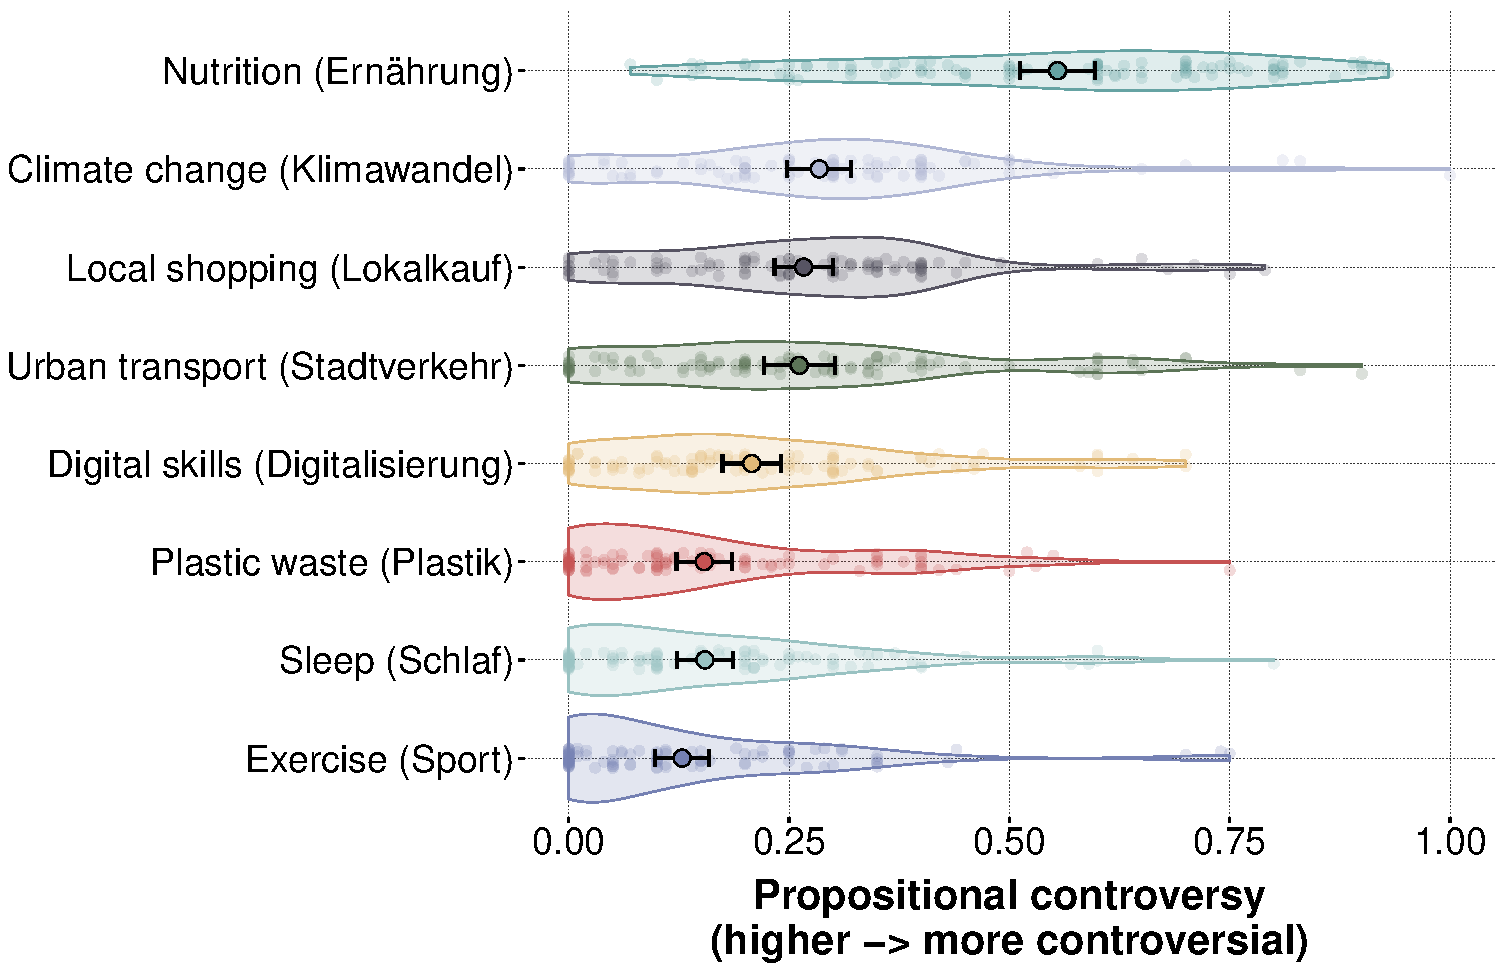
\includegraphics[width=\textwidth]{../../analysis/norming_exp/plots/norming_topic_means.pdf}
    \caption{Results of the norming experiment ($N\!=\!102$). German originals in parentheses.}\label{fig:norming}
  \end{subfigure}\hfill
  \begin{subfigure}[b]{0.49\textwidth}
    \centering
    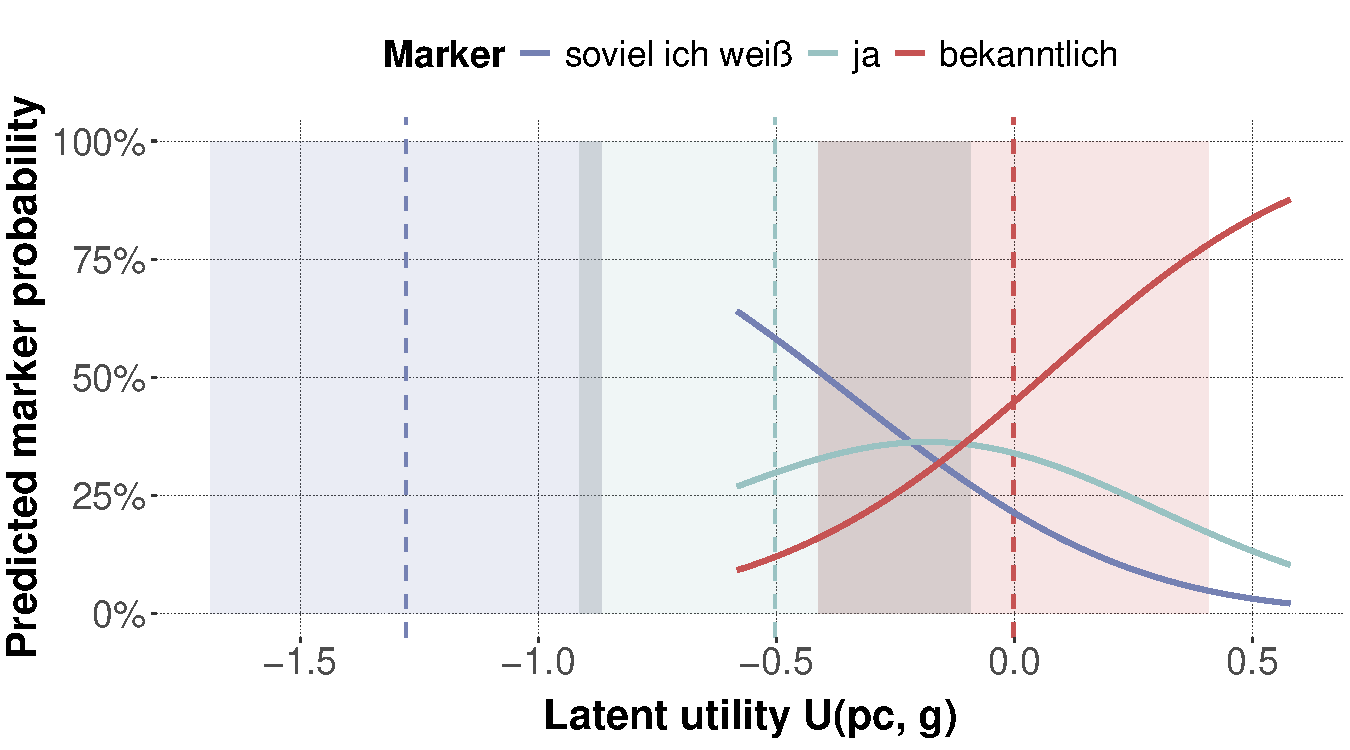
\includegraphics[width=\textwidth]{../../analysis/production_exp/plots/fig11_rsa_soft_thresholds.pdf}
    \caption{RSA noisy thresholds along the latent utility axis. Dashed lines: mean thresholds; shaded bands: overlapping regions. Because normed items are predominantly low-controversial, $pc_{\text{prop}}$ shifts the utility baseline well above the \textit{soviel ich wei\ss} (`as far as I know') threshold; the relevant variation thus falls mainly in the overlap zone between \textit{ja} (roughly `as you know') and \textit{bekanntlich} (`as is well known').}\label{fig:threshold}
  \end{subfigure}

  \smallskip

  \begin{subfigure}[b]{0.49\textwidth}
    \centering
    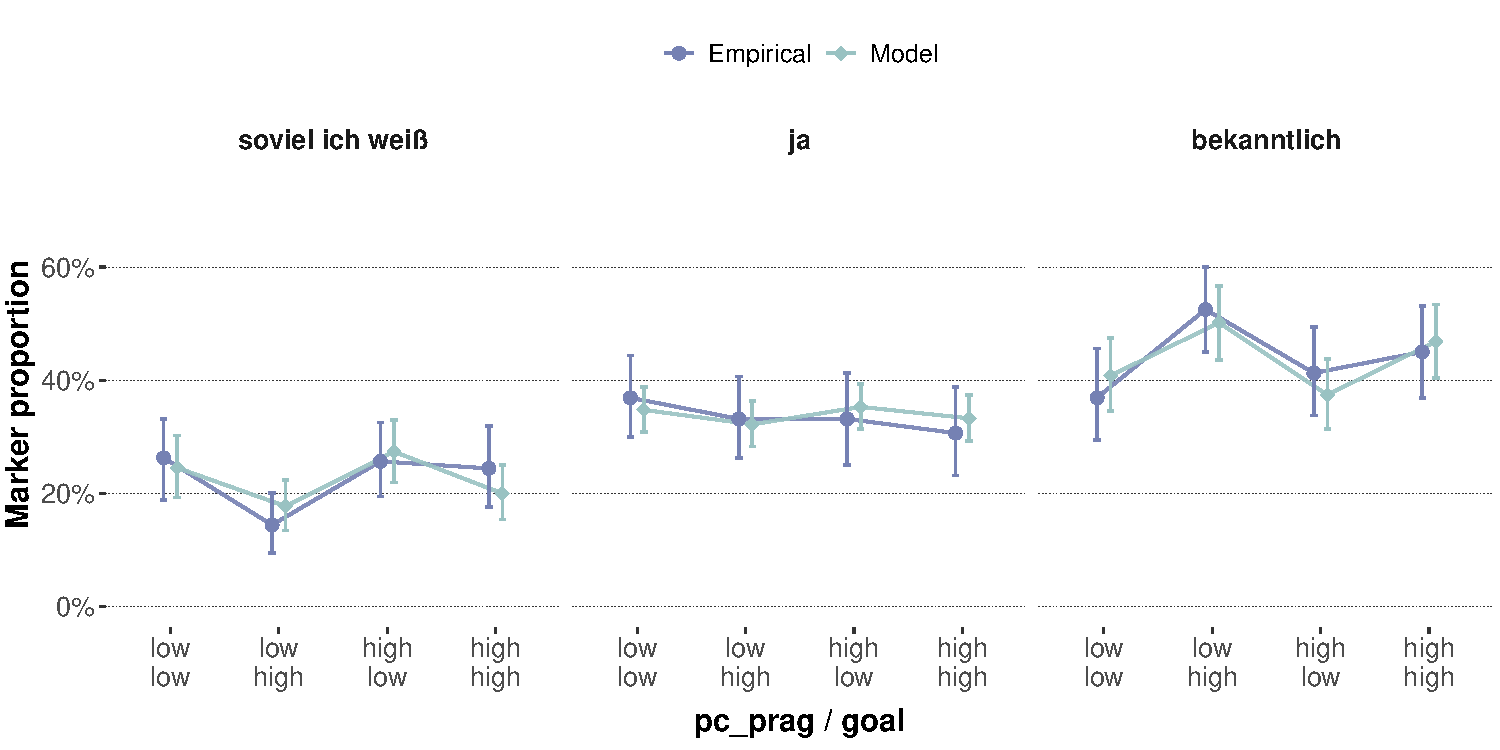
\includegraphics[width=\textwidth]{../../analysis/production_exp/plots/fig17c_facet_by_marker.pdf}
    \caption{Results of the production experiment ($N\!=\!80$).}\label{fig:production}
  \end{subfigure}\hfill
  \begin{subfigure}[b]{0.49\textwidth}
    \centering
    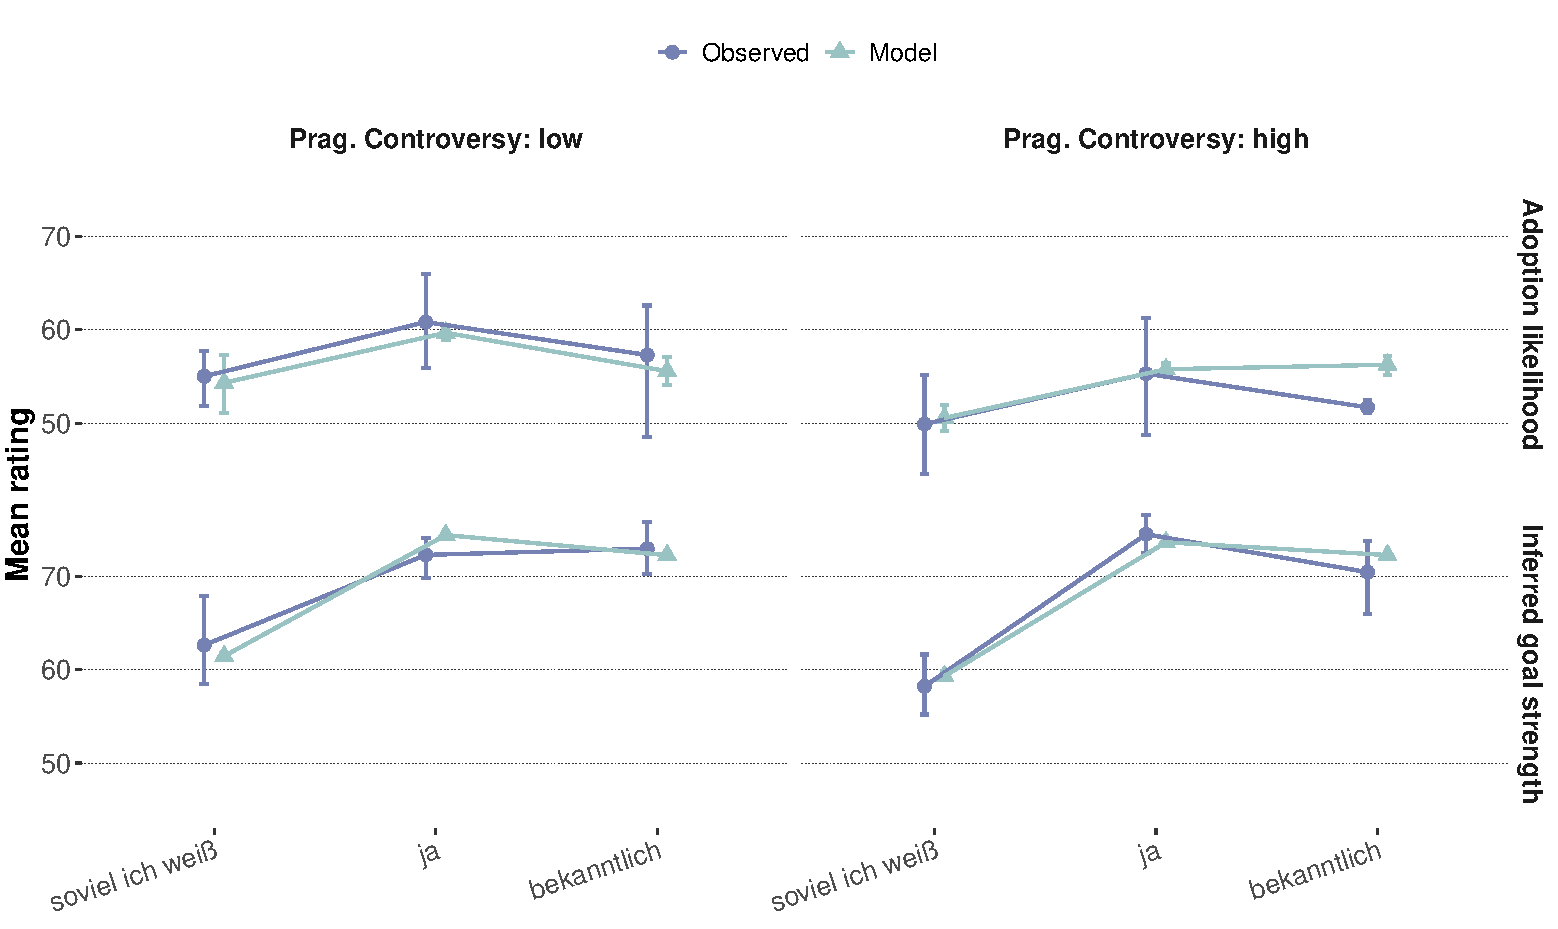
\includegraphics[width=\textwidth]{../../analysis/comprehension_exp/plots/fig7_rsa_base_vs_enhanced.pdf}
    \caption{Results of the comprehension experiment ($N\!=\!80$). Note that the production-trained model overestimates the effect of \textit{bekanntlich} (`as is well known') on adoption under high pragmatic controversy.}\label{fig:comprehension}
  \end{subfigure}

  \caption{Model and experimental results. Points show means; error bars show bootstrap 95\% confidence intervals.}
  \label{fig:all-results}
\end{figure}
\clearpage
\begin{figure}[h!]
  \centering
  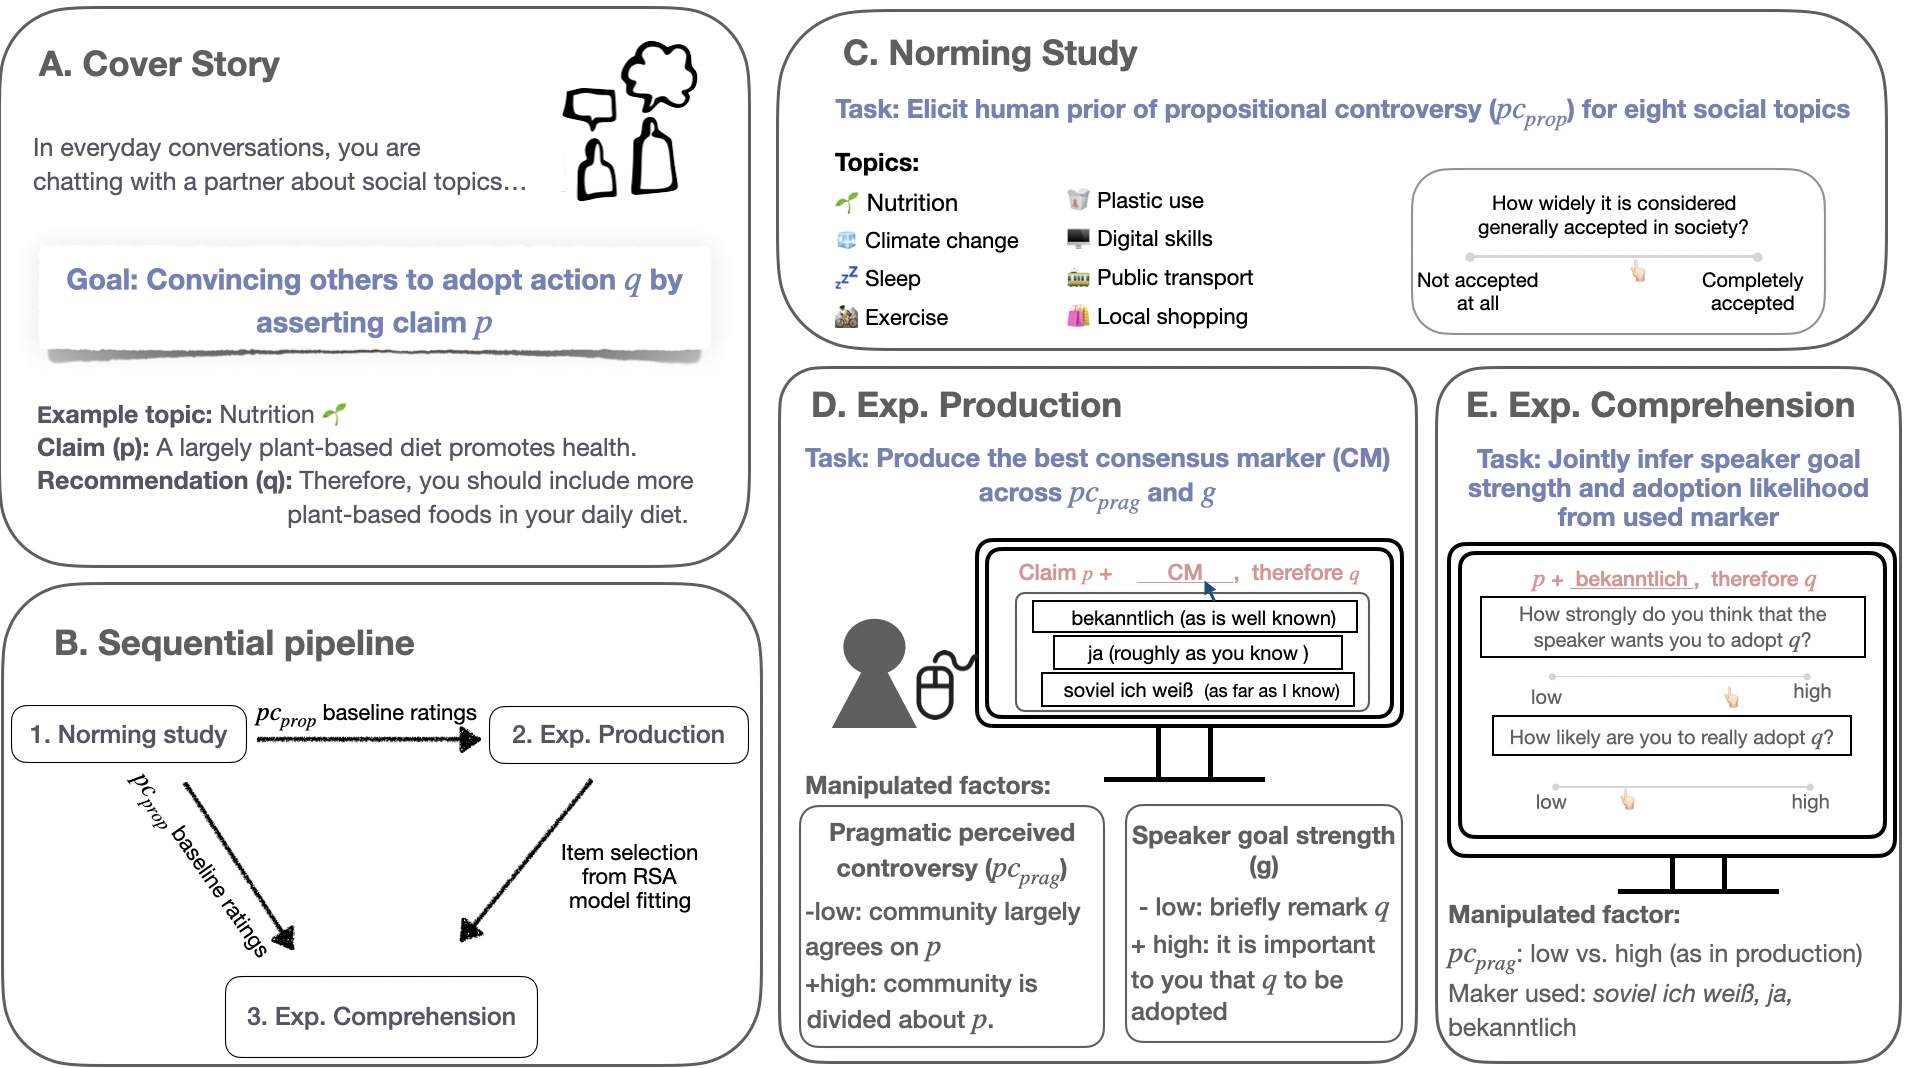
\includegraphics[width=\textwidth]{overview.png}
  \caption{Experimental pipeline. (A)~Cover story: participants discuss social topics with a partner, aiming to convince them to adopt a recommendation. (B)~Sequential design: a norming study establishes baseline propositional controversy, followed by production and comprehension experiments. (C)~Norming: eight topics rated for propositional controversy. (D)~Production: participants select the best consensus marker given manipulated pragmatic controversy and goal strength. (E)~Comprehension: participants infer speaker goal strength and adoption likelihood from marker-containing utterances.}
  \label{fig:overview}
\end{figure}

\textbf{References:}
\renewcommand{\bibsection}{}
{\footnotesize
\bibliographystyle{unsrtnat}
\bibliography{references}
}
\end{document}
